\documentclass[twocolumn]{aastex61}

\newcommand{\vdag}{(v)^\dagger}
\newcommand\aastex{AAS\TeX}
\newcommand\latex{La\TeX}

\newcommand{\project}[1]{\textsl{#1}}
\newcommand{\JWST}{\project{JWST}}
\newcommand{\HST}{\project{HST}}
\newcommand{\Spitzer}{\project{Spitzer}}

%% Reintroduced the \received and \accepted commands from AASTeX v5.2
%\received{July 1, 2016}
%\revised{September 27, 2016}
%\accepted{\today}
\submitjournal{ApJ}

\shorttitle{Phase Curves of WASP-103\lowercase{b}}
\shortauthors{Kreidberg et al.}

\begin{document}

\title{Global Climate and Atmosphere Composition of the Ultra-Hot Jupiter WASP-103\lowercase{b} from \HST\ and Spitzer Phase Curve Observations}

\correspondingauthor{Laura Kreidberg}
\email{laura.kreidberg@cfa.harvard.edu}

\author{Laura Kreidberg}
\affiliation{Harvard Society of Fellows\
78 Mt. Auburn St.\\
Cambridge, MA 02138, USA}
\affiliation{Harvard-Smithsonian Center for Astrophysics\
60 Garden St.\\
Cambridge, MA 02138}
\nocollaboration

\author{Vivien Parmentier}
\affiliation{Department of Planetary Sciences and Lunar and Planetary Laboratory, The University of Arizona}
\nocollaboration

\author{Michael R. Line}
\affiliation{Arizona State University}
\nocollaboration

\author{Kevin B. Stevenson}
\affiliation{Space Telescope Science Institute}
\nocollaboration

\author{Tom Louden}
\affiliation{University of Warwick}
\nocollaboration

\author{Mick\"{a}el Bonnefoy}
\affiliation{Universit\'{e} Grenoble Alpes}
\nocollaboration

\author{Jacqueline K. Faherty}
\affiliation{American Museum of Natural History}
\nocollaboration

\author{Gregory L. Henry}
\affiliation{Center of Excellence in Information Systems, Tennessee State University}
\nocollaboration

\author{Keivan Stassun}
\affiliation{Vanderbilt University}
\nocollaboration

\author{Jacob L. Bean}
\affiliation{University of Chicago}
\nocollaboration

\author{Jonathan Fortney}
\affiliation{University of California Santa Cruz}
\nocollaboration

\author{Adam Showman}
\affiliation{Department of Planetary Sciences and Lunar and Planetary Laboratory, The University of Arizona}
\nocollaboration

\author{Jean-Michel D\'{e}sert}
\affiliation{University of Amsterdam}

\begin{abstract}
WASP-103b is a short-period hot Jupiter.
\end{abstract}

\keywords{planets and satellites: individual (WASP-107b), planets and satellites: atmospheres}


\section{Introduction} \label{sec:intro}
The planets and moons of the Solar System possess a rich variety of -- weather, temperature var

It is a truism to say that planets are round.  The. And yet planets' roundness gives rise to a host of complications:  atmospheric circulation, variable , gradients in chemistry, cloud formation and evaporation, and time-dependent phenomena (weather).

It is a challenge is to reveal this structure at great distances, when we cannot spatially resolve the photosphere of the planet.  Most observations of exoplanet atmospheres are sensitive to a single isolated region  -- either the terminator, for transmission spectroscopy, or the disk-integrated dayside, for emission spectroscopy.  The solution to this problem is to observe phase curves of tidally-locked planets, which monitor the brightness of the planet over its entire orbit. As the orbital phase changes, the observer 

The first phase curve was observed with \Spitzer\ for the hot Jupiter HD 189733b by \citep{knutson??}, and was followed by FIXME more (with IRAC). Several trends emerged from these measurements, including eastward shifted hotspots (which suggest super-rotating equatorial jets), larger day-night temperature contrast for shorter period planets (ref), . The first spectroscopic phase curve was measured with Hubble's Wide Field Camera 3 (WFC3) by \citep{stevenson???} for the hot Jupiter WASP-43b. Found low albedo, offset hotspot, water visible at other phases, 

In parallel with these observations, there have been major advances in the theory of exoplanet atmospheres in three-dimensions. Global circulation models (GCMs) are now capable of self-consistent radiative transfer and atmospheric dynamics (refs) and are beginning to include clouds (refs?). 

In addition to GCMs, work on the inverse problem Cowan - how to get maps, . SPIDERMAN, an open-source Python package designed to take any temperature or brightness map of a planet and output the corresponding phase curve, so that we can readily connect GCMs to phase curve observations.  


In this paper we present \HST\ and \Spitzer\ phase curve observations of WASP-103b, a hot Jupiter with a mass of X, radius of Y, period of Z (cite discovery paper). These properties are similar to WASP-43b, except that WASP-103b has a much (FIXME vs FIXME K) thanks to its hot F?? star host. By comparing the phase curves of these two planets, we can test the effect of irradiation on the climate of the planet.

Talk about other WFC3 papers (Star Cartier, etc)

The structure of the paper is as follows:

\section{Observations and Data Reduction}
We observed two full-orbit phase curves of WASP-103b with \HST/WFC3 and one each with \Spitzer/IRAC at 3.6 and 4.5 $\mu$m (from HST Program 14050 and Spitzer Program 11099). We also reduced two \HST/WFC3 secondary eclipse observations of WASP-103b from \HST\ Program 13660 (PI: M. Zhao).

\subsection{\HST/WFC3}
The \HST\ phase curve observations consisted of two visits on 26-27 February and 2-3 August 2015. Each visit was 15 orbits in duration and spanned 23 hours. The last half of orbit 15 in each visit was used for a gyro bias update and does not produce useable science data.  We took a direct image of the star with the F126N filter at the beginning of each orbit to determine the wavelength solution zero-point. The remainder of the orbit consisted of time-series spectroscopy with the G141 grism ($1.1 - 1.7$ $\mu$m) and the 256 x 256 pixel subarray. We used the SPARS10/NSAMP = 15 read-out mode, which has an exposure time of 103 seconds. To optimize the duty cycle of the observations, we used the spatial scan observing mode with a scan rate of 0.03 arcsec/s, alternating between forward and backward scanning on the detector. The scan height was 25 pixels and the peak counts were $35\times10^3$ photoelectrons per pixel. We collected a total of 18 spatial scan exposures per orbit.  The two eclipse observations from Program 13660 had a similar observing setup.  

We reduced the data from both programs using a custom pipeline developed for past analyses of WFC3 data \citep[for details see][]{kreidberg14a, kreidberg14b, kreidberg15b}. Briefly, we use the optimal extraction algorithm of \cite{horne86} to extract each up-the-ramp sample (or ``stripe") separately. The stripes are then summed to create the final spectrum. For each stripe, the extraction window is 24 pixels high and centered on the stripe midpoint. We estimate the background from the median of a region of the detector that is uncontaminated by the target spectrum (rows 5-50). The typical background counts are low (10-15 photoelectrons per pixel, roughly 0.03\% of the peak counts from the target star). We note that the extracted spectrum includes flux from a nearby star, which is separated from WASP-103 by less than two pixels \citep[0.2";][]{wollert15}. Our extracted spectrum includes flux from this star, which we account for later in the analysis. 

\subsection{\Spitzer}
We also obtained \Spitzer/IRAC observations with 3.6 and 4.5 $\mu$m photometric filters (referred to as Channel 1 and Channel 2, respectively). The observations had the following setup. Each phase curve observation consisted of 30 hours of time series photometry, beginning three hours prior to one secondary eclipse and ending three hours after a second eclipse.  We used 12 s exposures to maximize the duty cycle without saturating the detector. The data volume is relatively low for this exposure time, so we read out the full array. To minimize the intrapixel effect (variations in flux caused by imprecise pointing), we did not dither and also used PCRS peak-up to improve the pointing accuracy. We began each observations with a 30-minute position settling period, followed by three Astronomical Observation Requests (AORs) of equal duration. At the beginning of each AOR, the telescope was repointed to position the target in the ``sweet spot" of the detector.

The data were reduced with the POET pipeline \citep{stevenson12}. We performed aperture photometry with an aperture size of 2.75 pixels (chosen from a grid of apertures between 2 and 4 pixels to minimize the residual noise in the light curve fits). We masked pixels that were flagged in the bad pixel mask provided in the ancillary data for the observations. The target centroid was determined with a two-dimensional Gaussian fit.  We estimated and subtracted the background from an annulus with a radius of 7 to 15 pixels from the centroid. As for the \HST\ observations, the contaminating flux from the nearby star is included in the final photometry and corrected later in the light curve fits.


\subsection{Photometric Monitoring}
We monitored WASP-103's photometric variability over 158 nights during 2014 - 2016 with the Tennessee State University Celestron 14-inch (C14) automated imaging telescope (AIT), located at Fairborn Observatory in southern Arizona \citep[][]{henry99}.  The observations of WASP-103 were made in the Cousins R passband with an SBIG STL-1001E CCD camera.  Each observation consisted of 4--10 consecutive exposures on WASP-103 along with several dozen comparison stars in the same field. The individual consecutive frames were co-added and reduced to differential magnitudes (i.e., WASP-103 minus the mean brightness of the six best comparison stars). The nightly observations were corrected for bias, flat-fielding, pier-side offset, and differential atmospheric extinction.  

The photometric analyses are summarized for each observing season in Table\,\ref{tab:photometry}.  The standard deviation of WASP-103's brightness in each season is given in column~4.  The mean of the three standard deviations is 0.0058~mag, which is very comparable to the mean standard deviation of the six comparison stars (0.0055~mag).  To maximize the possibility of detection WASP-103's rotation, we normalized the photometry such that each observing season has the same mean, thereby removing long-term variability in WASP-103 and/or the comparison stars. We performed a periodogram analysis of the normalized dataset. Figure\,\ref{fig:photometry} shows the frequency spectrum and the phase curve computed with the best frequency, respectively.  We also performed a least-squares fit to the data to determine the best fit sine curve. The best fit period is 6.814 days, which agrees closely with the estimated stellar rotation period of 6.855 days \citep{getal2014}.  The variability amplitude is 0.005~mag, which has FIXME impact on our analysis here.


\begin{figure}
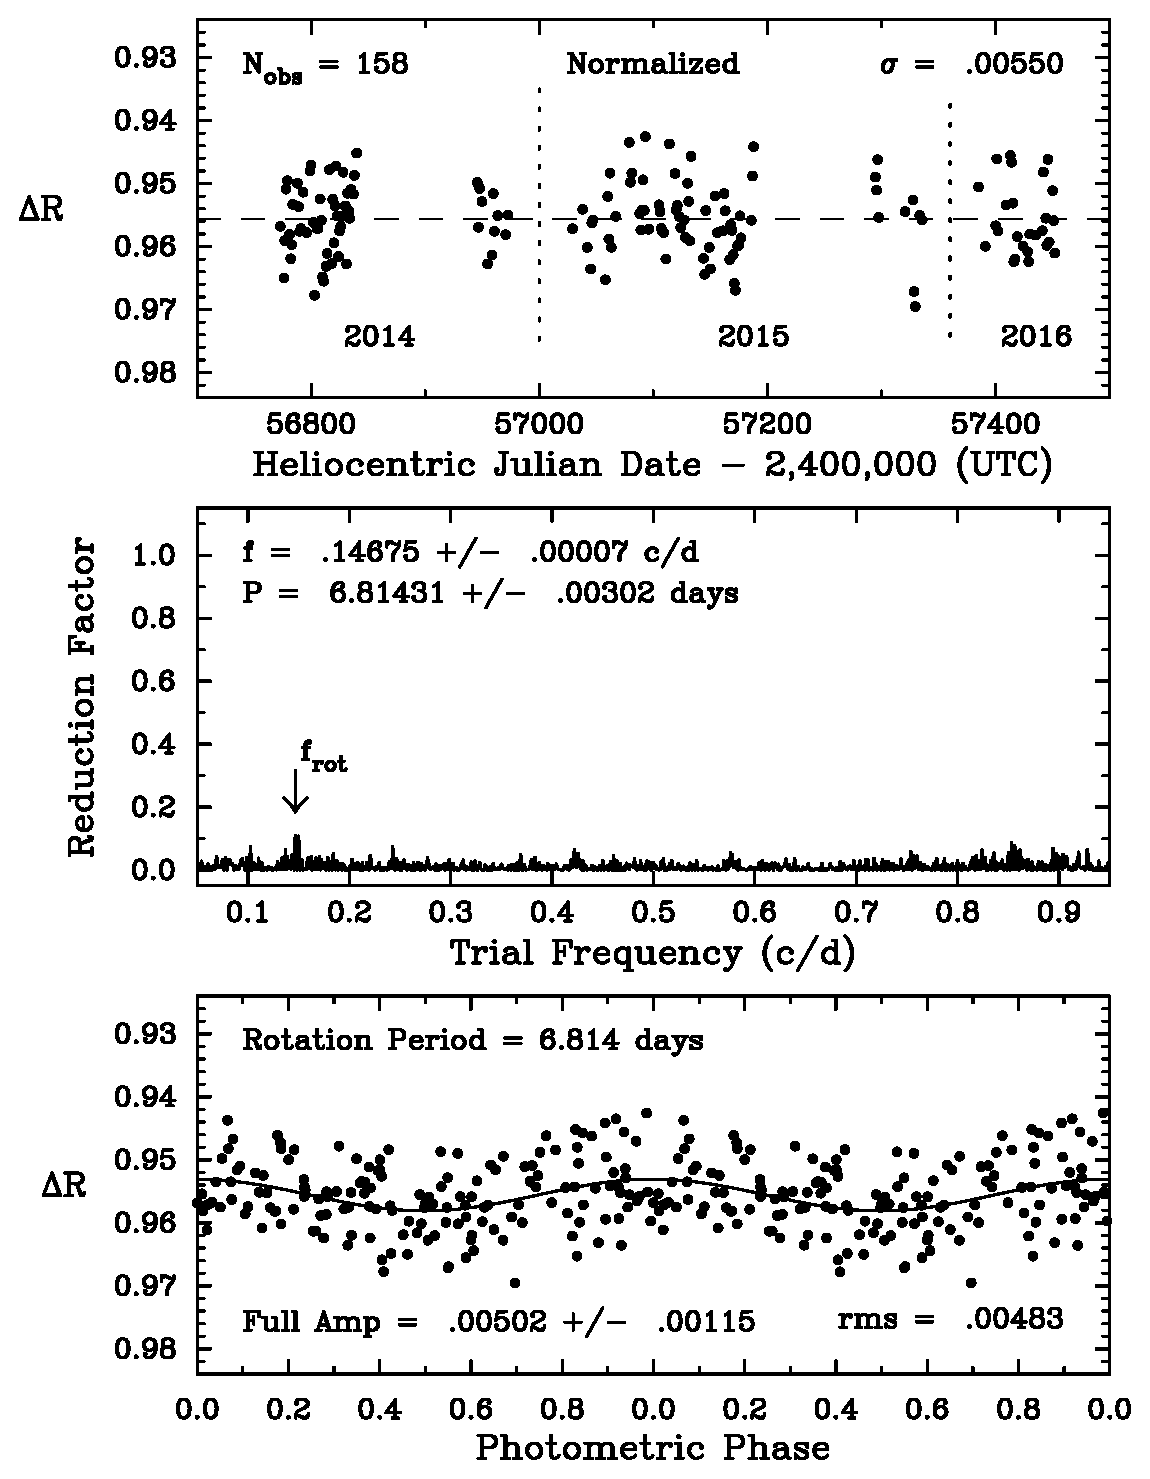
\includegraphics[width = 0.5\textwidth]{Figures/photometry.eps}
\caption{$Top$: The normalized nightly Cousins $R$ band photometric dataset for WASP-103, acquired with the C14 automated imaging telescope at Fairborn Observatory. Vertical dashed lines denote separate observing seasons. Gaps are due to target visibility and the Arizona monsoon season (July - September). $Middle$: The frequency spectrum of the normalized dataset suggests low-amplitude variability with a period of 6.814~days. $Bottom$: The normalized dataset phased to the 6.814-day period, which we interpret as the stellar rotation period. A least-squares sine fit to the 6.814-day rotation period gives a peak-to-peak amplitude of just 0.005~mag.}
\label{fig:photometry}
\end{figure}

\begin{deluxetable}{ccccc}
\label{tab:photometry}
	%\tabletypesize{\small}
	\tablenum{1}
	\tablewidth{0pt}
	\tablecaption{Photometric Observations of WASP-103}
	\tablehead{
		\colhead{Observing} & \colhead{} & \colhead{Date Range} &
	\colhead{Sigma} & \colhead{Seasonal Mean} }% \\

%		\colhead{Season} & \colhead{$N_{obs}$} & \colhead{(HJD $-$ 2,400,000)} &
%		\colhead{(mag)} & \colhead{(mag)}}%   \\

	%	\colhead{(1)} & \colhead{(2)} & \colhead{(3)} &
	%	\colhead{(4)} & \colhead{(5)}  
	\startdata
	   2014   &  59 & 56722--56972 & 0.0057 & $0.9546\pm0.0007$  \\
	   2015   &  73 & 57028--57335 & 0.0062 & $0.9549\pm0.0007$  \\
	   2016   &  26 & 57385--57451 & 0.0055 & $0.9485\pm0.0011$  \\
	\enddata
\end{deluxetable}


\section{Light Curve Fits}
We fit a two-component model to the light curves. One component models the astrophysical signal (the planet's thermal phase variation and transit), and the other component models the systematic noise introduced by time-dependent changes in instrument performance. For each light curve, we fit the physical and systematic components simultaneously, such that the total observed flux as a function of time is given by $F(t) = F_\mathrm{physical}(t) \times F_\mathrm{sys}(t)$. For the \HST\ data, where we observed two phase curves and two additional eclipses, we constrain the physical parameters to be the same for all visits, but allow some of the systematics parameters to vary (for more details see \S\,\ref{sec:hst_sys}). We fit the WFC3 band-integrated (``white" light curve"), as well as spectroscopic light curves created from 10 wavelength bins uniformly spaced at $0.05\,\mu$m intervals between $1.15$ and $1.65\,\mu$m.

\subsection{Astrophysical Signal}
We assume the measured astrophysical signal $F_\mathrm{physical}$ has the following form:
\begin{equation}
	%F_\mathrm{physical}(\lambda, t) = F_s(\lambda) (1 + \alpha(\lambda)) \times T(\lambda, t) + F_p(\lambda, t) 
	F_\mathrm{physical}(\lambda, t) =  T(\lambda, t) + c(\lambda, t) \times F_p/F_s(\lambda, t)
\end{equation}
where $T(\lambda, t)$ is the transit model (the fraction of the stellar disk that is visible at time $t$), $F_p/F_s(\lambda, t)$ is the disk-integrated planet-to-star flux, and $c$ is a correction factor for companion star dilution and the planet's tidal distortion. 

We calculated the transit model $T(t)$ with the \texttt{batman} package \citep{kreidberg15a}. Many of the physical parameters are tightly constrained by \cite{southworth15}, so we fixed the orbital period, time of inferior conjunction, orbital inclination, and ratio of semi-major axis to stellar radius to the previously published values ($P = 0.925545613$ day, $t_0 = 2456836.2964455\,\mathrm{BJD_{TDB}}$, $i = 87.3^\circ$, and $a/R_s = 2.999$). As a test, we fit for these parameters with the Spitzer Channel 2 light curve, which has the best phase coverage and least systematic noise of the three data sets. We found that the transit parameters are consistent with the \cite{southworth15} results, so we proceeded with the remainder of the analysis holding those parameters fixed.  The free parameters for the transit model were the transit depth $r_p$ and a linear limb darkening parameter $u$. 

We calculated the planet-to-star flux $F_p/F_s$ in two different ways. First, we fit a sinusoid with a period equal to the planet's orbital period. The free parameters were the sine curve amplitude and phase offset. For the second approach, we used the \texttt{SPIDERMAN} package \citep{louden17} to model $F_p/F_s$. This package allows users to input a climate map (temperature or brightness as a function of latitude and longitude), and generate the corresponding flux ratio for an observation at time $t$. In our fit, we calculated the stellar flux with a PHOENIX model \citep{husser13} interpolated to an effective temperature of $6110\,\mathrm{K}$ \citep{gillon14}.  For the planet flux, we tested three different maps: a two-temperature map, with a uniform dayside temperature $T_d$ and a uniform nightside temperature $T_n$; a map generated with spherical harmonics; and the physically-motivated kinematic model from \cite{zhang17}, which has just three free parameters (the nightside temperature $T_n$, the change in temperature from day-to-night side $\Delta_T$, and the ratio of radiative to advective timescales $\xi$).  In all cases, we assumed that the planet is tidally locked, such that each orbital revolution corresponds to one complete rotation on its spin axis. 

We scaled the planet-to-star flux by a correction factor $c$ to account for dilution from the companion star and ellipsoidal variability due to the planet's tidal distortion. The correction factor took the form: 
\begin{equation}
	c(\lambda, t) = [1 + \alpha(\lambda)]A(t)
\end{equation}
where $\alpha(\lambda)$ is the additional fractional flux from the companion star and $A(t)$ is the sky-projected area of the planet. We estimated $\alpha(\lambda)$ based on the best fit spectral energy distribution from \cite{cartier17}. The companion star contributes $10-16\%$ of the flux over the wavelength range $1 - 5\,\mu$m.  We calculated $A(t)$ using the analytic formula from \cite{leconte11b}, equation B.9, which computes the projected area of a triaxial ellipsoid. We estimated the ellipsoid properties using Table B.3 of \cite{leconte11a}, assuming the planet radius is 1.5 $R_\mathrm{Jup}$ and age is 5 Gyr. The predicted ellipsoidal variability is shown in Figure\,\ref{fig:ellipsoidal}. At quadrature, the projected radius is $8\%$ larger than at phase zero (mid-transit). %FIXME: say this doesn't matter.
%In addition to temperature, the planet's visible surface area $[R(t)]^2$ is also expected to vary with orbital phase due to tidal distortion \citep{gillon14}. In the observed light curve, changes in planet radius are degenerate with changes in temperature. 

%We explored adding an additional sine term to model the thermal phase variation, but the additional degrees of freedom are not justified according to the Bayesian Information Criterion (BIC). 


%Our light curves are not precise enough to detect the ellipsoidal variability, but we include a model prediction $E(t)$ to avoid introducing any bias in the thermal phase variation. We model $E(t)$ using the analytic expression from \cite{leconte11}, which 
%FIXME doppler beaming?

\begin{figure}
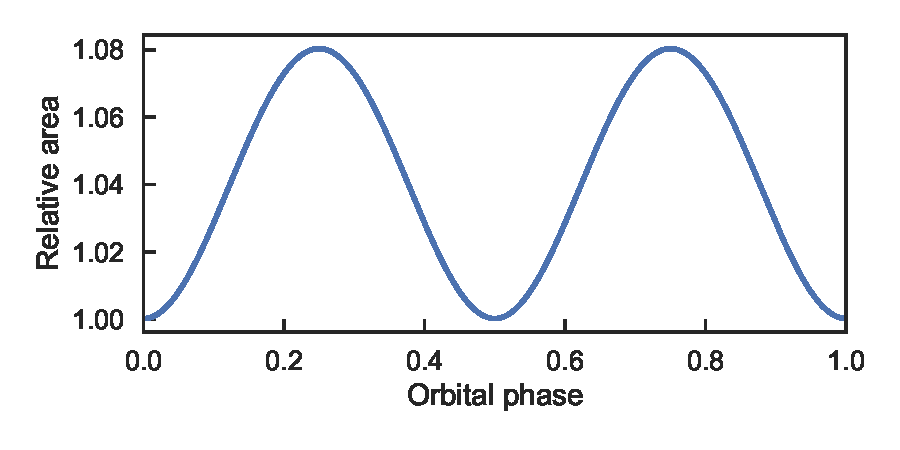
\includegraphics[width = 0.5\textwidth]{Figures/ellipsoidal.pdf}
\caption{Projected area of the planet as a function of orbital phase, normalized to unity at phase zero. The area variation was predicted analytically using the model from \cite{leconte11b}.}
\label{fig:ellipsoidal}
\end{figure}

\begin{figure}
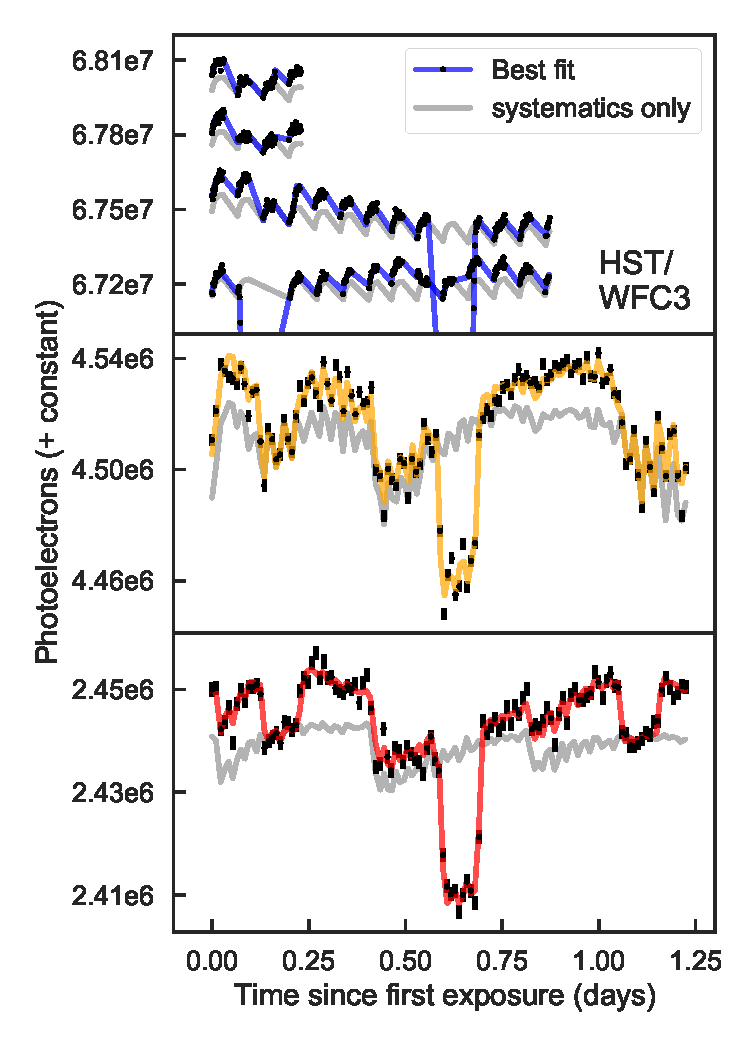
\includegraphics[width = 0.5\textwidth]{Figures/systematics.pdf}
\caption{Raw light curves for WASP-103b observed with \HST/WFC3 (top panel) and \Spitzer/IRAC (bottom two panels). The data points are indicated with black dots. The \HST\ data are unbinned, and the Spitzer data are binned in time segments of 15 minutes with error bars indicating the bin standard deviation. The colored lines show the best fit models, which include the astrophysical signal and instrument systematics. The gray lines indicate the contribution from the instrument systematics alone (which would be observed for a source with constant brightness and no planet). For visual clarity, we corrected the \HST\ data for the upstream-downstream effect, separated the four visits by adding a flux offset, and zoomed in on the phase variation, so the transits are not displayed in the panel.}
\label{fig:systematics}
\end{figure}


\subsection{Systematics}
Both the \HST\ and \Spitzer\ phase curves have systematic noise caused by variations in the sensitivity of the instrument over time. For the \HST/WFC3 data, the dominant systematic is an orbit-long exponential trend due to charge traps filling up over successive exposures \citep{long15, zhou17}. For \Spitzer\, the primary source of noise is the intrapixel sensitivity effect. The detector's pixels do not have uniform sensitivity, so slight changes in telescope pointing cause the recorded flux to vary. In Figure\,\ref{fig:systematics}, we show the raw light curves before systematic noise was removed. The systematics have comparable amplitude to the thermal phase variation signal, so they must be carefully corrected to recover the underlying planet-to-star flux. 

\subsubsection{\HST\ Systematics}
\label{sec:hst_sys}
We fit the WFC3 systematics using an analytic model of the form:
\begin{equation}
 F_\mathrm{sys}(t) = (c\,S(t) + v_1\,t_\mathrm{v} + v_2\,t_\mathrm{v}^2)(1 - \exp(-a\,t_\mathrm{orb} - b))
\end{equation}
where $t_\mathrm{v}$ is time elapsed since the first exposure in a visit and $t_\mathrm{orb}$ is time since the first exposure in an orbit. $S(t)$ is a scale factor equal to 1 for exposures with spatial scanning in the forward direction and $s$ for reverse scans, to account for the upstream-downstream effect \citep{mccullough12}. The orbit-long ramp parameters are consistent for all the visits, so we constrained $a$, $b$, and $s$ to have the same value for all visits in the final fit. The visit-long trends differ from visit to visit, so $c$, $v_1$, and $v_2$ were allowed to vary between visits. We fixed $v_2$ to zero for the two secondary eclipse observations from Program 13360, since the visit-long trend for shorter observations is fit well by a linear slope.

Some segments of the data exhibit stronger systematics than others, so we exclude these data in our final analysis. We drop the first orbit from every visit and the first exposure from every orbit \citep[following common practice; see e.g.][]{kreidberg14a}.  We also discard exposures from the last half of orbit 15 from the phase curve observations, which were taken in staring mode to enable a gyro bias update. Since we observed two phase curves, we have complete orbital phase coverage the planet despite discarding some data.

\subsubsection{\Spitzer\ Systematics}
We fit the \Spitzer\ systematics with the POET pipeline, which uses the BLISS mapping technique \citep{stevenson12}. This approach creates a map of the intrapixel sensitivity while simultaneously fitting for other systematics and the physical parameters of the system. The sensitivity map is determined by bilinear interpolation over a grid of knots centered on the stellar flux. Each knot's sensitivity is calculated from the residuals to the light curve fit: the higher the flux values for data points near a given knot, the higher the detector sensitivity is at that position.  To avoid overfitting, we chose the grid scale such that bilinear interpolation performed better than nearest neighbor interpolation. For the $3.6\,\mu$m data, the grid scale was 0.008 pixel in both $x$ and $y$. For $4.5\,\mu$m, the scale was 0.022 pixel.  

In addition to the intrapixel sensitivity variation, we fit the data for a linear trend in time. We tested a quadratic trend but did not find significant evidence for the additional model complexity based on the Bayesian information criterion (BIC). 

As discussed in \S \ref{sec:fitquality}, the 3.6 $\mu$m light curve exhibits time correlated noise. To account for this additional source of error, we fit the wavelet model from \cite{carter09} (simultaneously with the other fit parameters). FIXME: describe wavelets.


\begin{figure*}
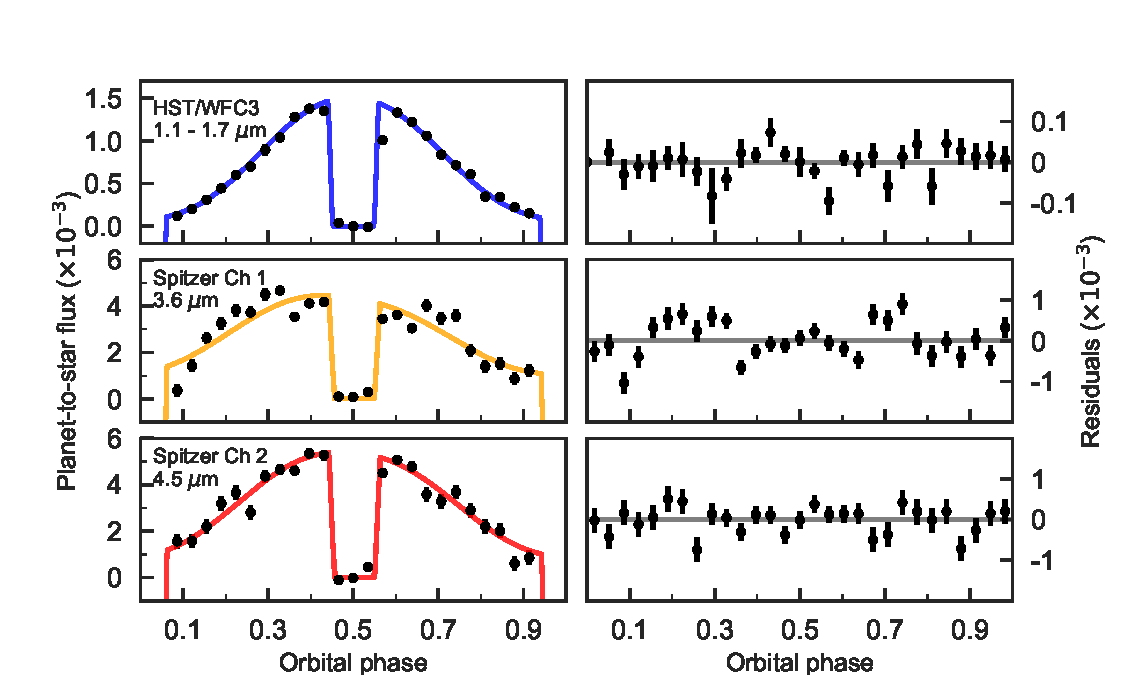
\includegraphics[width = 1.0\textwidth]{Figures/phase_curves_spherical.pdf}
\caption{WASP-103b phase curve observations from \HST/WFC3 (top) and \Spitzer/IRAC (middle and bottom). For clarity, the data are phase-folded on the planet's orbital period and binned in 30 uniformly spaced bins between 0 and 1. The left column shows the phase curves with systematic noise removed (black points) compared to the best fit spherical harmonics model (colored lines). The error bars denote $1\,\sigma$ uncertainties (in some cases, the errors are smaller than the data points).
%The shading denotes the  1\,$\sigma$ confidence interval on the best fit. 
We include the transits in the fit, but they are not displayed in this figure. The right-hand column shows the binned residuals for the best-fit light curve.}
\label{fig:phasecurves}
\end{figure*}

\section{Results}
The fitted light curves are shown in Figure\,\ref{fig:phasecurves}. This figure shows results from the kinematic model for the thermal phase variation and has instrument systematics removed.  Broadly speaking, the phase curves show large amplitude phase variation, ranging from 1.5 parts-per-thousand (ppt) in the WFC3 bandpass to 5 ppt in \Spitzer\ Channel 2.  The planet flux changes significantly with orbital phase in all three of the data sets, suggesting a strong gradient from dayside to nightside temperature. The peak brightness occurs near phase 0.5.
In this section we discuss the quality 

\subsection{Goodness of Fit}
\label{sec:fitquality}
We performed several tests of the quality of the light curve fits.  First we predicted the level of scatter in the light curves based on photon noise alone, then compared this value to the root-mean-square (rms) of the fit residuals.  The Spitzer 4.5 $\mu$m light curve rms is within 10\% of the expected photon noise limit (691 versus 640 ppm), whereas the 3.6 $\mu$m light curve has significantly larger rms (797 versus 470 ppm), due to time-correlated red noise (discussed below). The expected photon-limited rms for the WFC3 spectrosopic light curves ranges from 430 - 530 parts per million (ppm), and the measured rms was typically within 5\% of expectations for all spectroscopic channels.  For the WFC3 band- integrated white light curve, the rms was slightly larger than predicted (175 versus 122 ppm). There are a number of possible origins for this discrepancy, including imperfect background subtraction, variation in the position of the spatial scan on the detector, loss of flux outside the extraction window, and imperfect modeling of the astrophysical signal or instrument systematics. However, our analysis of the composition and thermal structure of the planet's atmosphere is based on the wavelength-dependent data (which reach the photon limit), so we do not further explore the small excess noise in the white light curve. 

%Spitzer expected rms calculated from Figures/systematics.py
%Ch1: rms obs, exp (ppm) 796.931457529 470.309808368
%Ch2: rms obs, exp (ppm) 691.221416885 639.675550854

In addition to calculated the fit rms compared to the photon noise, we also tested for the presence of red noise based on whether the rms decreases as expected when the light curve in binned in time.  If the noise is white (uncorrelated in time), the residuals are expected to decrease by a factor of $\sqrt{N}$, where $N$ is the number of points in a bin. Figure\,\ref{fig:rms} shows the binned residuals compared to expectations for white noise. The \HST/WFC3 and \Spitzer\ Channel 2 light curves agree well with expectations, whereas \Spitzer\ Channel 1 shows higher noise than expected as bin size increases. This test confirms the presence of time-correlated noise in the Channel 1 light curve that can be seen by eye in the residuals in Figure\,\ref{fig:phasecurves}. Both \Spitzer\ channels use the same detector, but Channel 1 data are more susceptible to time-correlated noise because the the point spread function is narrower at shorter wavelengths, making intrapixel sensitivity variations more pronounced.

The reduced $\chi^2$ values for the fits are near unity. FIXME when you have them all.
%Third, we calculated several goodness of fit statistics. $\chi^2$, AIC, BIC.

\begin{figure}
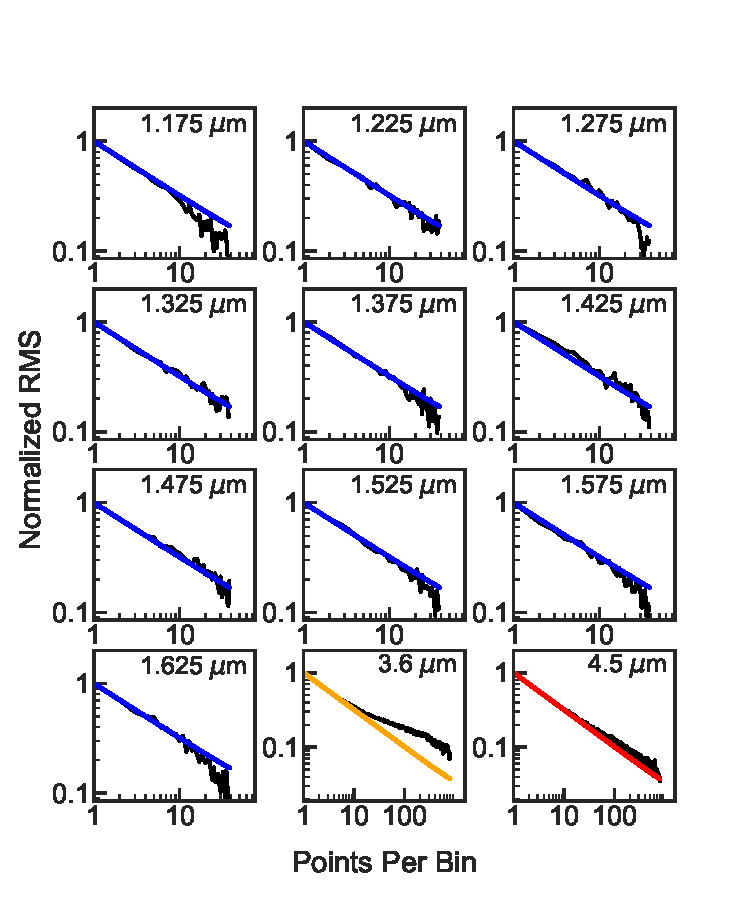
\includegraphics[width = 0.5\textwidth]{Figures/rms.pdf}
\caption{Root mean square (rms) variability in the light curves as a function of bin size (black lines) compared to the expected rms from photon noise (colored lines). The central wavelength of the light curve is indicated in the upper right corner of each panel. With the exception of the \Spitzer\ 3.6 $\mu$m channel, the rms for the light curves bins down in agreement with predictions from the photon noise.}
\label{fig:rms}
\end{figure}

\begin{deluxetable}{llllll}
\label{tab:model_comparison}
	\tablecolumns{6}
	\tablewidth{0pt}:
	\tablecaption{Model Comparison \label{table:models}}
	\tablehead{\colhead{Data} & \colhead{Model} & \colhead{$T_\mathrm{min}$} & \colhead{$T_\mathrm{max}$} & \colhead{$\Delta_\mathrm{AIC}$} & \colhead{$\Delta_\mathrm{BIC}$}}
		\startdata
		WFC3 & Sph. Harmonics & 1214 & 3251 & 0.0 & 0.0 \\
		\, & Kinematic & 1980 & 3958 & 11.8 & 11.8 \\
		\, & Two Temp. & 0 & 2887 & 47.7 & 43.2 \\
		\, & Sinusoid & -- & -- & 17.7 & 13.2 \\
		Ch 1 & Sph. Harmonics & 1280 & 3444 & 48.0 & 0.0 \\
		\, & Kinematic & 1955 & 3675 & 82.3 & 34.3 \\
		\, & Two Temp. & 1429 & 3041 & 58.7 & 17.6 \\
		\, & Sinusoid & -- & -- & 0.0 & 98.4 \\
		Ch 2 & Sph. Harmonics & 902 & 3786 & 2.2 & 3.1 \\
		\, & Kinematic & 1703 & 4276 & 16.55 & 17.41 \\
		\, & Two Temp. & 1361 & 3311 & 26.1 & 0.0 \\
		\, & Sinusoid & -- & -- & 0.0 & 49.6 \\
		\enddata
		\vspace{-0.8cm}
		\tablecomments{comments}
\end{deluxetable}

\subsection{Phase-Resolved Spectra}
We used the best-fit phase curves (with systematics removed) to generate phase-resolved emission spectra.  Since our model does not fit eclipse depth as a free parameter, we estimated the dayside emission spectrum as follows. We used \texttt{SPIDERMAN}'s eclipse\_depth method to calculate the average planet-to-star flux for the best-fit model during secondary eclipse.  To estimate uncertainties, we took the standard deviation of the residuals of the in-eclipse data points, then added this value in quadrature to the standard deviation of the residuals of the out-of-eclipse data.  This quadrature sum accounts for the uncertainty in the baseline flux. To account for red noise in the \Spitzer\ $3.6\,\mu$ light curve, we use the approach of \cite{pont06} to determine the red noise contribution on the timescale of the eclipse. We add the estimated red noise in quadrature, which increases the uncertainty on planet-to-star flux by a factor of $2.5$.

For the other orbital phases, we binned the light curve (with systematics removed) in eight intervals of about 0.1 in orbital phase, with endpoints at phases $0.06, 0.15, 0.25, 0.35, 0.44$ and $0.56, 0.65, 0.75, 0.85, 0.94$. These endpoints were chosen to ensure that there is no contribution from in-transit or in-eclipse data.  In each phase bin, we estimated the planet-to-star flux from the mean value of the data points in the bin. To estimate the uncertainty, we took the standard deviation of the points in the bin and added it in quadrature to the standard deviation of the data points during secondary eclipse (phase $0.46-0.54$), to account for the uncertainty in baseline stellar flux.  For the $3.6\mu$m data, we also add red noise on the timescale of a phase bin, following \cite{pont06}.  The phase-resolved emission spectra are shown in Figure\,\ref{fig:spectra} and listed in Table\,\ref{table:spectra}. 

To test that the phase-resolved spectra are robust to different approaches for fitting the data, we compared the spectra for all four of the thermal phase variation models (sinusoid, kinematic, spherical harmonics, and two temperature). We found that the choice of model does not significantly change the results.  The emission spectra are insensitive to the models because they are estimated directly from the data (after systematics have been removed). Since systematic noise is not strongly correlated with the astrophysical signal, the systematics-divided data are nearly identical for all the models.  This point is illustrated in Figure\,\ref{fig:model_comparison} for the broadband WFC3 light curve. In most phase bins, the planet-to-star flux agrees to well within one sigma for all the models. 


\begin{figure*}
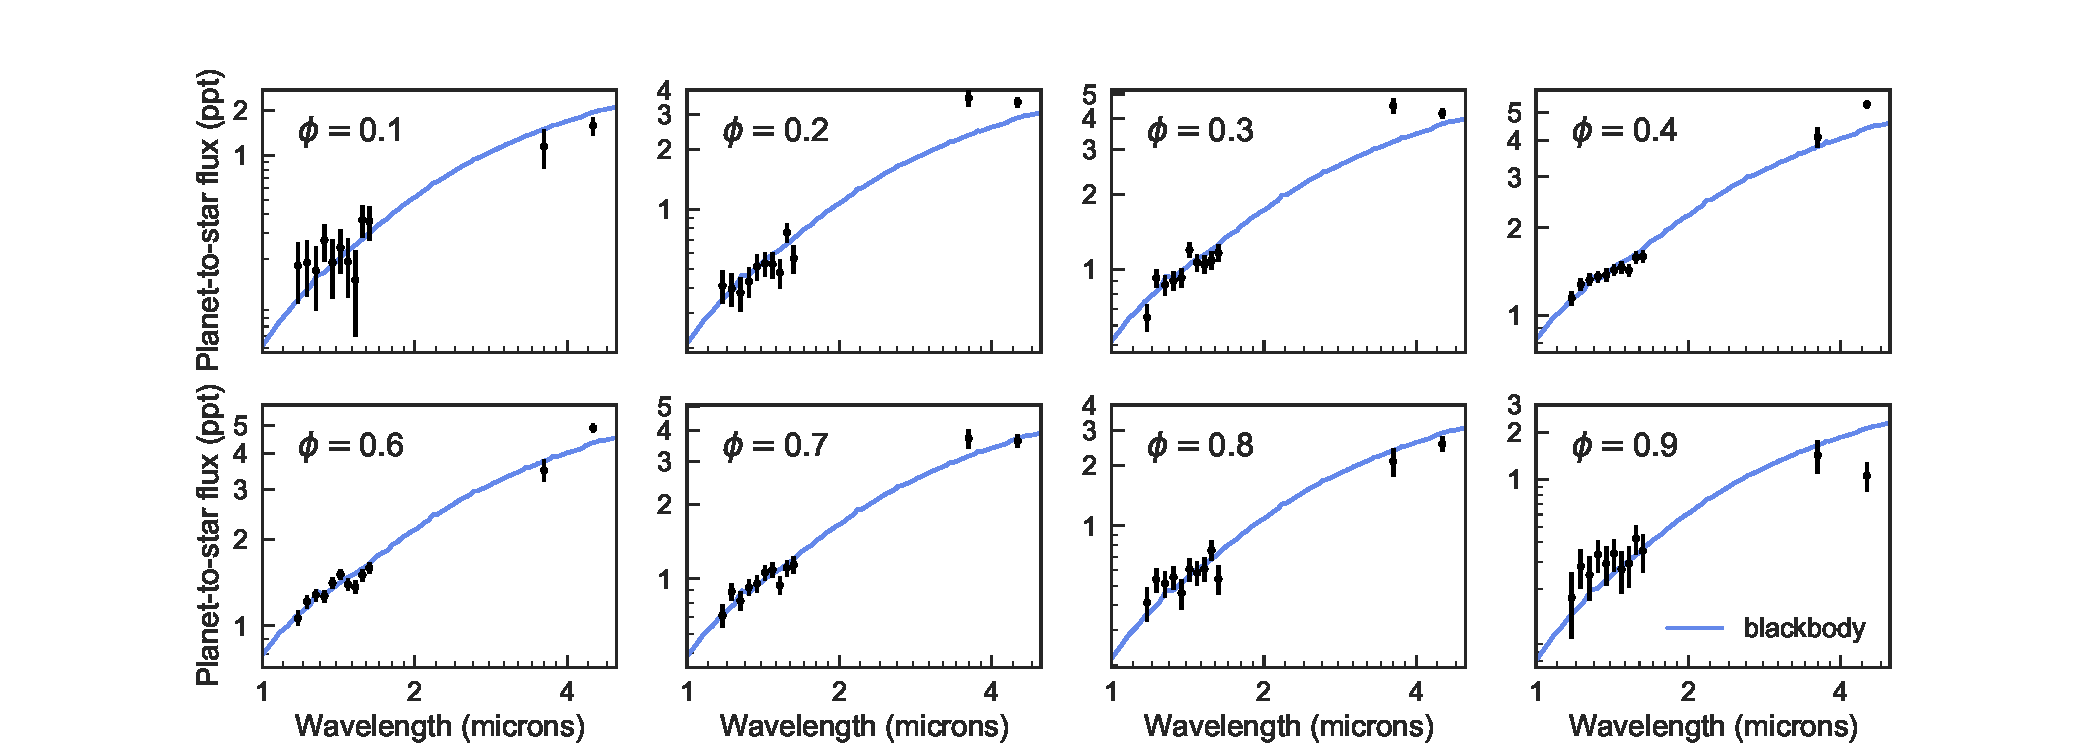
\includegraphics[width = 1.0\textwidth]{Figures/emission_spectra.pdf}
\caption{Phase-resolved emission spectra (points) compared to the best fit blackbody (blue line) and the GCM with $\tau_\mathrm{drag} = 10^3$ s. Phases $\phi = 0.5$ and $0.0$ are centered on the substellar and anti-stellar points, respectively.}
\label{fig:spectra}
\end{figure*}

\begin{figure*}
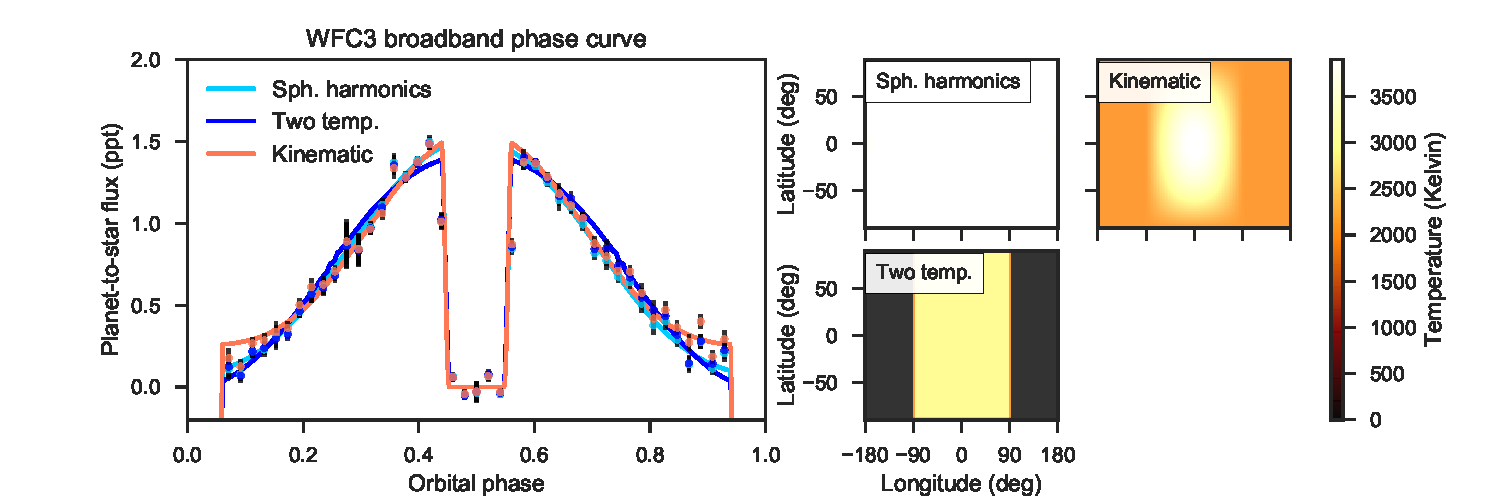
\includegraphics[width = 1.0\textwidth]{Figures/hst_model_comparison.pdf}
\caption{\textbf{Left:} Fits to the broadband WFC3 phase curve compared to a GCM. The colored lines correspond to different temperature maps fit to the data, and the dashed gray line is from the $\tau_\mathrm{drag} = 10^3$ GCM. We also show the planet-to-star flux corresponding to each map (points), which is model-dependent due to slight degeneracies with the instrument systematic model.  \textbf{Right:} Temperature maps from the best fit models and the GCM at 0.1 bar.}
\label{fig:model_comparison}
\end{figure*}

\begin{deluxetable*}{lllllllllll}
	\tablecolumns{11}
	\tablewidth{0pt}:
	\tablecaption{Phase-Resolved Emission Spectra \label{table:spectra}}
	\tablehead{
	\colhead{$\lambda$} & \colhead{Dilution} & \colhead{$\phi = 0.1$} & \colhead{$\phi = 0.2$} & \colhead{$\phi = 0.3$} & \colhead{$\phi = 0.4$} & \colhead{$\phi = 0.5$} & \colhead{$\phi = 0.6$} & \colhead{$\phi = 0.7$} & \colhead{$\phi = 0.8$} & \colhead{$\phi = 0.9$}}
		\startdata
		1.175 & 0.10 & $ 179 \pm 79 $ & $ 411 \pm 77 $ & $ 647 \pm 80 $ & $ 1143 \pm 65 $ & $ 1259 \pm 47 $ & $ 1063 \pm 64 $ & $ 710 \pm 73 $ & $ 412 \pm 78 $ & $ 177 \pm 79 $ \\ 
		1.225 & 0.11 & $ 188 \pm 76 $ & $ 398 \pm 74 $ & $ 928 \pm 77 $ & $ 1276 \pm 62 $ & $ 1448 \pm 46 $ & $ 1216 \pm 62 $ & $ 888 \pm 71 $ & $ 539 \pm 75 $ & $ 280 \pm 76 $ \\ 
		1.275 & 0.11 & $ 166 \pm 76 $ & $ 379 \pm 74 $ & $ 869 \pm 77 $ & $ 1323 \pm 62 $ & $ 1480 \pm 46 $ & $ 1282 \pm 62 $ & $ 814 \pm 71 $ & $ 515 \pm 75 $ & $ 247 \pm 76 $ \\ 
		1.325 & 0.11 & $ 266 \pm 75 $ & $ 432 \pm 73 $ & $ 904 \pm 76 $ & $ 1357 \pm 62 $ & $ 1498 \pm 45 $ & $ 1267 \pm 61 $ & $ 925 \pm 70 $ & $ 552 \pm 74 $ & $ 333 \pm 75 $ \\ 
		1.375 & 0.12 & $ 189 \pm 81 $ & $ 514 \pm 78 $ & $ 928 \pm 82 $ & $ 1376 \pm 66 $ & $ 1611 \pm 48 $ & $ 1411 \pm 65 $ & $ 954 \pm 75 $ & $ 461 \pm 79 $ & $ 292 \pm 81 $ \\ 
		1.425 & 0.13 & $ 238 \pm 79 $ & $ 532 \pm 76 $ & $ 1198 \pm 79 $ & $ 1431 \pm 64 $ & $ 1718 \pm 47 $ & $ 1511 \pm 64 $ & $ 1063 \pm 73 $ & $ 605 \pm 77 $ & $ 338 \pm 79 $ \\ 
		1.475 & 0.14 & $ 191 \pm 81 $ & $ 527 \pm 79 $ & $ 1068 \pm 82 $ & $ 1460 \pm 66 $ & $ 1667 \pm 48 $ & $ 1392 \pm 66 $ & $ 1090 \pm 75 $ & $ 580 \pm 80 $ & $ 268 \pm 81 $ \\ 
		1.525 & 0.14 & $ 143 \pm 84 $ & $ 478 \pm 81 $ & $ 1048 \pm 85 $ & $ 1429 \pm 69 $ & $ 1623 \pm 50 $ & $ 1367 \pm 68 $ & $ 943 \pm 77 $ & $ 607 \pm 82 $ & $ 291 \pm 84 $ \\ 
		1.575 & 0.15 & $ 367 \pm 88 $ & $ 761 \pm 85 $ & $ 1088 \pm 89 $ & $ 1581 \pm 72 $ & $ 1749 \pm 52 $ & $ 1503 \pm 71 $ & $ 1107 \pm 81 $ & $ 754 \pm 86 $ & $ 422 \pm 88 $ \\ 
		1.625 & 0.16 & $ 359 \pm 93 $ & $ 565 \pm 90 $ & $ 1169 \pm 94 $ & $ 1590 \pm 76 $ & $ 1843 \pm 56 $ & $ 1593 \pm 75 $ & $ 1142 \pm 86 $ & $ 542 \pm 91 $ & $ 351 \pm 93 $ \\ 
		3.6 & 0.17 & $ 1148 \pm 333 $ & $ 3633 \pm 330 $ & $ 4487 \pm 320 $ & $ 4107 \pm 314 $ & $ 4458 \pm 383 $ & $ 3495 \pm 315 $ & $ 3720 \pm 330 $ & $ 2102 \pm 331 $ & $ 1431 \pm 334 $ \\ 
		4.5 & 0.16 & $ 1586 \pm 220 $ & $ 3468 \pm 214 $ & $ 4188 \pm 190 $ & $ 5334 \pm 179 $ & $ 5686 \pm 138 $ & $ 4904 \pm 183 $ & $ 3626 \pm 214 $ & $ 2575 \pm 217 $ & $ 1057 \pm 221 $ \\ 
		\enddata
		\vspace{-0.8cm}
		\tablecomments{comments}
	\end{deluxetable*}


\begin{figure}
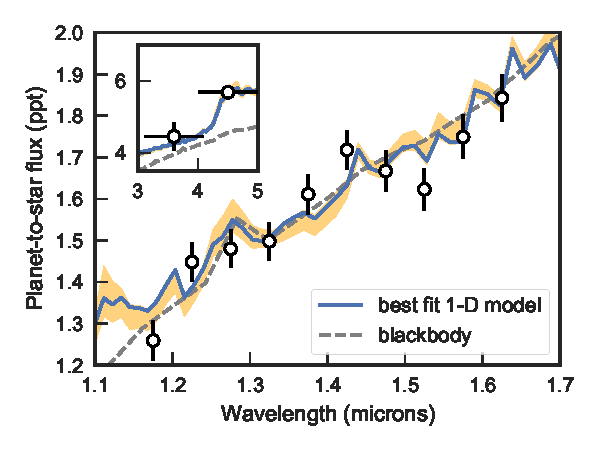
\includegraphics[width = 0.5\textwidth]{Figures/dayside_spectrum.pdf}
\caption{Dayside emission spectrum (points) compared to the best fit 1-D model (blue line) with $1\,\sigma$ uncertainty shaded in orange. We also show the best fit blackbody (fit to the WFC3 data only).}
\label{fig:dayside}
\end{figure}


\subsection{Comparison of Thermal Phase Variation Models}
We compared four different models for the thermal phase variation: a sinusoid and three temperature maps. The sinusoid has been widely used to model phase variation in previous analyses \citep[e.g.][]{knutson09, stevenson14}. One advantage of the sinusoid model is that it directly fits the phase variation amplitude and offset from the substellar point, and can be inverted to map the climate \citep{cowan08}. Fitting temperature maps directly is a new approach enabled by the \texttt{SPIDERMAN} package.  We consider three parameterizations for the temperature map, which each have different strengths. One is a physically-motivated kinematic model that closely reproduces GCM simulations \citep{zhang17}.  The second parameterization is a spherical harmonic map, which is the most flexible model we consider and makes the fewest assumptions about the true climate. The third model has just two free parameters, a dayside temperature and a nightside temperature. This model is easiest to compare to one-dimensional forward models of the dayside, which assume a uniform temperature/pressure profile.  

All of the models provide reasonable fits to the data, with $\chi^2_\nu$ near unity, but they yield significantly different temperature maps. Table\,\ref{tab:model_comparison} lists the minimum and maximum temperatures for the best fit models to the WFC3 broadband and two Spitzer phase curves. We also list the  information criterion (BIC) and Aikike information criterion (AIC) values for the fits \citep[a $\Delta$BIC value greater than 10 constitutes strong evidence against a given model;][]{kass95}.

%Both of these statistics are an approximation of the Bayesian evidence for a given model, but the BIC penalizes model complexity relatively more than the AIC \citep{kass95}. 

The best fit model is either a sinusoid or spherical harmonics, depending on which criterion is used for model selection. The BIC generally favors the simpler spherical harmonics model because it penalizes model complexity relatively more than the AIC \citep{kass95}. The sinusoid has eight free parameters (amplitude, phase offset, eclipse duration, ingress/egress duration, and midpoint and depth for each of two eclipses), whereas the spherical harmonics model has four (for degree two).  The kinematic and two temperature models tend to perform significantly worse ($\Delta$BIC and $\Delta$AIC greater than 10).  As illustrated in Figure\,\ref{fig:model_comparison}, the kinematic model overpredicts the nightside flux, whereas the two temperature model overpredicts the flux at quadrature and underpredicts the dayside. 
%The spherical harmonics model is strongly favored for most of the data sets according to the AIC and BIC. It has slightly more free parameters than the other models (four, versus three for the kinematic model and two for the two-temperature model). 

We compared the planet's minimum and maximum temperature for the three climate maps by computing the temperatures over a $100\times100$ grid in latitude and longitude. The kinematic model has the hottest dayside temperature and the two-temperature model has the smallest. The differences in peak temperature for the models we consider ranges from $630\,\mathrm{K}$ for \Spitzer\ Channel 1 to $1070\,\mathrm{K}$ for the broadband WFC3 light curve. The minimum nightside temperature is also model-dependent: for the WFC3 data, the two-temperature model predicts a nightside temperature of zero Kelvin, whereas the best fit kinematic model has a nightside temperature of $1980\,\mathrm{K}$. %For the WFC3 data, the peak temperature ranges from $2890$ to $3960$ K, and the minimum ranges from $0$ to $1980$ K.  

These differences arise because the kinematic model allows a steep temperature gradient on the dayside, so the substellar point is much hotter than the terminator, whereas the two temperature map imposes a constant dayside temperature.  The spherical harmonics model has an intermediate temperature gradient, and fits the data the best. However, this model may not be physically realistic: on the nightside, it produces higher temperatures at the poles than at the equator, contrary to predictions from GCMs (which we discuss in \S\,\ref{sec:gcm}). 

%The typical uncertainty is FIXME (run MCMC, say the systematic range is larger than the error bars). 

%The spherical harmonics model fits better according to the BIC and the AIC; however, it yields higher temperatures at the poles than at the equator, which does not agree with predictions from GCM simulations \citep{FIXME}. 


\subsection{Hotspot Offset}
The location of peak brightness of the phase curve is a proxy for the efficiency of thermal reradiation to space and relative to heat transport by advection (the radiative-to-advective timescale). The faster the reradiation, the less heat can be redistributed to the nightside. We compared the measured hotspot offset for the different models and found FIXME.

%\subsection{Clouds?}


\section{Atmospheric Composition and Thermal Structure}
\label{sec:composition}
To interpret the phase-resolved spectra, we performed two model fits. First, we modeled the planet flux as a simple blackbody to estimate the dayside brightness temperature and test for significant absorption or emission features. We then performed a more sophisticated grid-based retrieval to evaluate the atmospheric composition and thermal structure. 

\subsection{Blackbody Fits}
A blackbody is the simplest model for the planet's thermal emission and provide a useful first evaluation of the atmospheric properties. The best fit blackbodies are shown in Figures \ref{fig:spectra} and \ref{fig:dayside}. This model performs well for some orbital phases, with $\chi^2_\nu$ ranging from 0.9 to 1.1 for phases $\phi = 0.1, 0.7$ and $0.8$. At other phases the blackbody model is a poorer fit, particularly to the \Spitzer\ data. For phases $0.2 - 0.6$, the \Spitzer\ eclipse depths are larger than predicted for the best fit blackbody, suggesting the presence of an emission feature. On the nightside (phase $0.9$), the \Spitzer\ $4.5\,\mu$m eclipse depth is \emph{smaller} than predicted, suggesting an absorption feature. These differences hint at changing thermal structure with longitude in the atmosphere.

We also fit blackbody models to the WFC3 data only, and found that they provide a good fit at all orbital phases. The $\chi^2_\nu$ values range from 0.5 to 1.6, with a median of 0.9. The best fit effective temperatures range from 1920 Kelvin on the nightside to 2980 Kelvin on the dayside. We report the best fit temperatures with uncertainties in Table\,\ref{table:teffs}.  The dayside spectrum is the poorest fit by the blackbody model. This finding is not a surprise because the dayside has higher signal-to-noise than the other orbital phases, thanks to the two secondary eclipse observations from \cite{cartier17}. The more sophisticated grid-based retrieval provides a better fit to the dayside.

\begin{deluxetable}{lll}
	\tablecolumns{3}
	\tablewidth{0pt}:
	\tablecaption{Phase-resolved Effective Temperature \label{table:teffs}}
	\tablehead{
	\colhead{Phase} & \colhead{Effective Temperature} & \colhead{$\chi^2_\nu$}}
		\startdata
		0.1 & $ 1919 \pm 40 $ & 0.6 \\
		0.2 & $ 2256 \pm 24 $ & 0.8 \\
		0.3 & $ 2651 \pm 17 $ & 1.2 \\
		0.4 & $ 2906 \pm 11 $ & 0.8 \\
		0.5 & $ 3013 \pm 8 $ & 1.6 \\
		0.6 & $ 2885 \pm 12 $ & 1.3 \\
		0.7 & $ 2636 \pm 16 $ & 0.9 \\
		0.8 & $ 2313 \pm 23 $ & 1.1 \\
		0.9 & $ 2027 \pm 36 $ & 0.5 \\
		\enddata
		\vspace{-0.8cm}
		\tablecomments{comments}
	\end{deluxetable}
%Over the WFC3 bandpass, the phase-resolved spectra are featureless and consistent with blackbodies (with best fit $\chi^2_\nu$ ranging from $0.5-1.3$). However, the \Spitzer\ data, particularly at 4.5 $\mu$m, are discrepant with the best fit blackbody by $3-5\,\sigma$ at most orbital phases, indicating the presence of infrared molecular absorption or emission features. We investigate possible atmospheric compositions and temperature structures in \S\,\ref{sec:composition}. 

\subsection{Grid-Based Retrieval}
Since the phase-resolved spectra do not show spectrally resolved molecular features, we opted for a simple grid-based fit to the planet's atmospheric properties, similar to the grid search used in Mansfield et al. and Arcangeli et al. (in prep). We generated a grid from one-dimensional forward models of the atmosphere over a broad range of metallicities, carbon-to-oxygen ratios (C/O), and stellar irradiation. The stellar spectrum is scaled in intensity over the grid to model the unknown heat redistribution for the planet; i.e., a lower dayside irradiation is equivalent to more efficient heat transport to the nightside. 

At each point in the grid, we compute forward models to determine self-consistent, radiative-convective temperature-pressure (T-P) profiles. We determine the molecular abundances in each atmospheric layer assuming thermochemical equilibrium.  We include opacity from the major absorbers expected for a hot Jupiter atmosphere, including H$_2$O, CO, CO$_2$, TiO, and VO (\textbf{Mike: what others?}). Notably, in contrast to many previous studies of the hottest planets, we also included opacity from H-, which is expected because water dissociates at dayside photospheric temperature and pressure (3000 K, 0.1 bar).  Using these opacities and T-P profiles, we calculated thermal emission spectra over the full grid using the CHIMERA retrieval suite.  We then explored the grid with an MCMC chain using the \texttt{emcee} package \citep{foremanmackey13}, and interpolated in the grid to calculate the likelihood at each model step. We fit this model to the dayside and nightside emission spectra (phases $\phi = 0.5$ and $0.1$). 

\begin{figure}
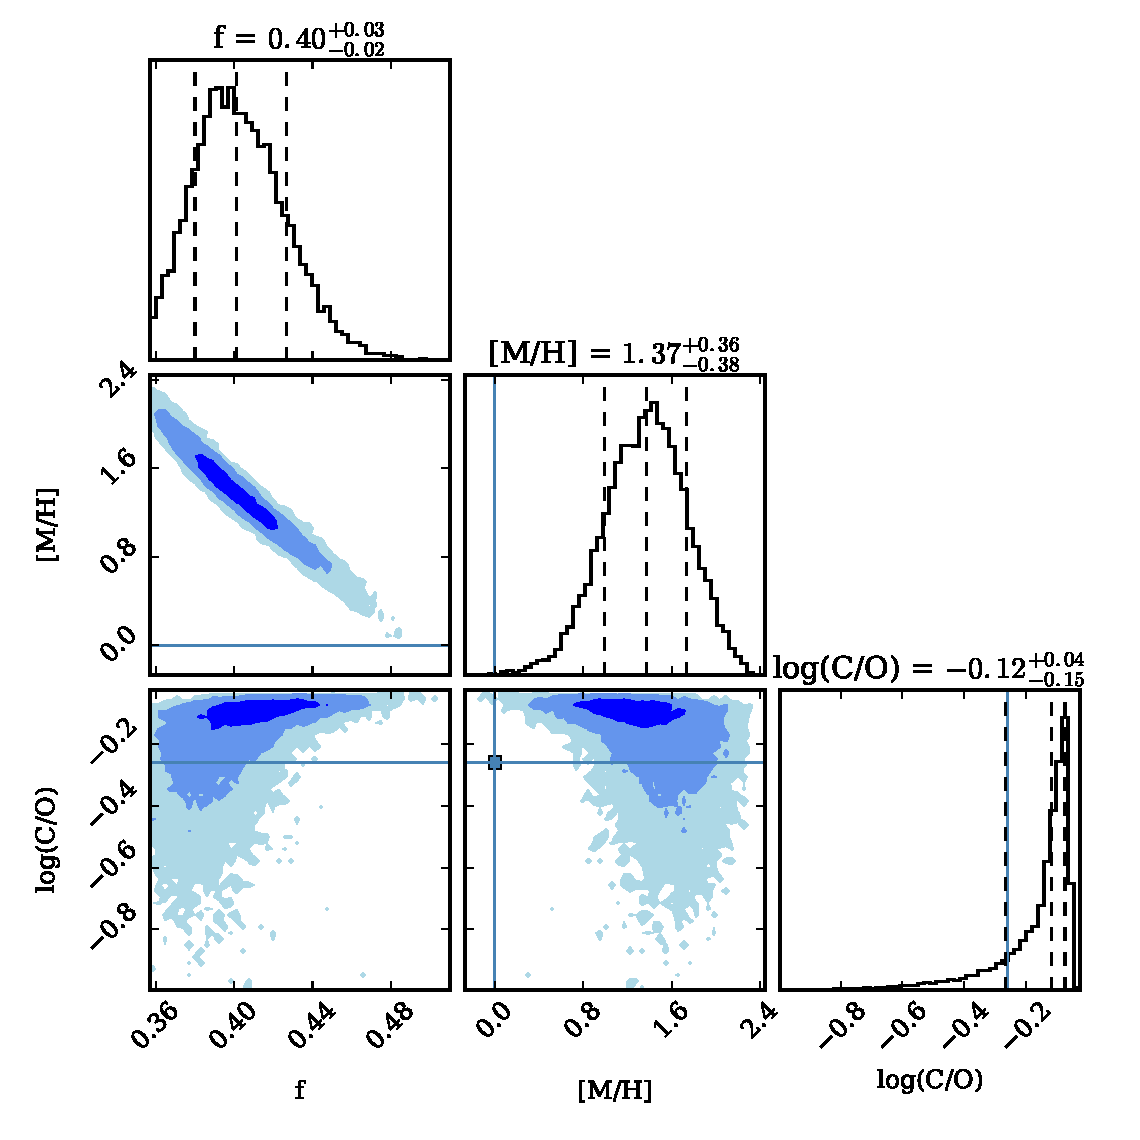
\includegraphics[width = 0.5\textwidth]{Figures/WASP-103b_grid_DAYSIDE_stair_pairs_02.pdf}
\caption{Posterior distributions for WASP-103b's atmospheric heat redistribution, metallicity, and C/O, from a grid-based fit to the dayside emission spectrum. The histograms on the diagonal show the marginalized distribution of each parameter, with dashed lines indicating the median and surrounding 68\% confidence interval. \textbf{Mike: what percentiles does the colored shading correspond to?} The blue lines correspond to solar metallicity (1) and C/O (0.54).}
\label{fig:composition}
\end{figure}

\subsubsection{Dayside Spectrum}
The main characteristics of the dayside emission spectrum are: (1) it is blackbody-like at WFC3 wavelengths, and (2) in the \Spitzer\ bands, the planet-to-star flux is significantly higher than predicted for the best fit blackbody, indicating an emission feature.  The best fit spectrum reproduces these data fairly well, with $\chi^2_\nu$ = 1.77. The WFC3 and Spitzer $3.6\,\mu$m points are fit better ($\chi^2_\nu$  = 1.17 for these data alone), but the $4.5\,\mu$m point is higher than the best fit model by $2.9\,\sigma$.  The best fit model has a moderately enhanced metallicity ($23\times$ solar), carbon-to-oxygen equal to 0.76, poor heat redistribution, and a thermal inversion (temperature increasing with altitude).

Figure\,\ref{fig:opacities} shows the opacity contributions of key absorbers for the best fit.  In the optical (which we do not observe directly), there is strong absorption by TiO/VO.  In the near-infrared, the dominant absorbers are H$_2$O and H-.  The observed spectrum is featureless at these wavelengths, due to a combination of factors: water is partially dissociated in the photosphere, leading to a drop in abundance of FIXME.  It also produces H- opacity (single H atoms bind with free electrons), which dominates spectral features from H$_2$O at wavelengths shorter than FIXME $\mu$m.  Water is also an efficient coolant, so lower water abundance leads to a more isothermal photosphere and weakens the features even more.  Taken together, all these factors conspire to produce a nearly featureless spectrum from $1.1 - 1.7\,\mu$m. Finally, in the infrared the dominant absorber is CO, which produces the emission feature at \Spitzer\ wavelengths.  

The TiO/VO absorption heats the upper atmosphere, resulting in a thermal inversion. Figure\,\ref{fig:TP} shows a selection of 100 randomly selected dayside T-P profiles. The profiles are nearly isothermal over a pressure range of $1-10^{-2}$ bars, with a median temperature near 2900 Kelvin. The temperature increases over $10^{-2} - 10^{-3}$ bars to 3500 Kelvin, and then begins to decrease again at pressures below $10^{-3}$ bar. (\textbf{Mike: what are the contribution functions?}). 


In Figure\,\ref{fig:composition}, we show the posterior distributions from the grid retrieval.  We infer a range in metallicity of $23^{+29}_{-13}\times$ solar, somewhat higher than expected based on Jupiter's metal enrichment \citep[$3-5\times$ solar;][]{wong04} and the trend toward decreasing metallicity with increasing planet mass observed for the Solar System and exoplanets \cite[e.g.][]{kreidberg14b}.  However, planet population synthesis models predict some scatter in atmospheric metallicity. Planets near WASP-103b's mass ($1.5\,M_\mathrm{Jup}$) are expected to have metallicities ranging from roughly $1-10\times$ solar \citep{mordasini16}. Our result for WASP-103b lies on the upper end of this range, and may be indicative of intrinsic scatter in the mass-atmospheric metallicity relation. 

The retrieved C/O is consistent with solar, with a $1\sigma$ confidence interval of $0.54 - 0.85$. We infer an upper limit on C/O of 0.9 at $3\,\sigma$ confidence, driven by the fact that the atmospheric chemistry is expected to change dramatically when C/O exceeds unity. For a carbon-rich composition, the equilibrium abundance of methane relative to CO increases by orders of magnitude compared to an oxygen-rich  composition \citep[e.g.][]{madhusudhan11}. Our \Spitzer\ eclipse depths are sensitive to the relative abundance of these species, so we can confidently rule out a carbon-rich composition in spite of the lack of spectrally resolved features.  

We infer a heat redistribution $f = 0.4^{+0.03}_{-0.02}$. The $f$ parameter is allowed to range from 0 (isotropic heat distribution) to 0.5 (dayside emission only). Our estimate of $f$ is close to the maximum, indicating inefficient transport of heat to the nightside. Poor heat transport is observed in other very hot planets as well, due to damping of heat-propagating waves by fast radiative cooling or frictional drag in a partially ionized atmosphere \citep{komacek16}. The heat redistribution is correlated with atmospheric metallicity (\textbf{Mike: why is this?}).  

We note that an important caveat for our results is that the best fit model is not a perfect fit to the data (with $\chi_\nu = 1.77$), so the uncertainties produced by the MCMC may be underestimated. Furthermore, the inferred C/O and metallicity are highly sensitive to the planet-to-star flux at \Spitzer\ $4.5\,\mu$m, which is the worst fit data point. To fit this data point, the model favors super-solar metallicities and C/O, which drive up the CO abundance (the dominant absorber at $4.5\,\mu$m). Given that the result hinges on a single photometric band and there are no spectrally resolved molecular features to constrain the temperature-pressure profile or which absorbers are present, we caution against over-interpreting these results until wider spectral coverage is available.
%As a test of our modeling approach, we also performed a retrieval in which the T/P profile was allowed to vary. 

\begin{figure}
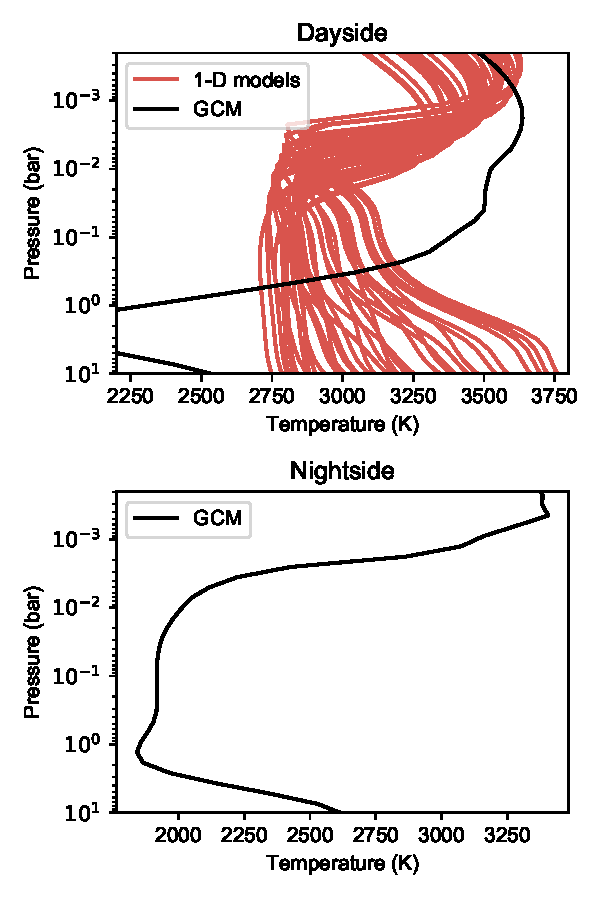
\includegraphics[width = 0.5\textwidth]{Figures/TP.pdf}
\caption{Dayside temperature-pressure profiles from the grid retrieval (red lines) compared to the profile from the substellar point for the FIXME GCM.}
\label{fig:TP}
\end{figure}

\subsubsection{Nightside Spectrum}
We also fit the nightside spectrum (phase $0.1$) with the grid-based retrieval. The best fit spectrum has a non-inverted temperature pressure profile.  At 1\,$\sigma$ confidence, the metallicity is $15 - 240\times$ solar and the C/O is unbounded over the full prior range (\textbf{Mike: what priors did you use?}). The atmospheric composition is consistent with results from the dayside spectrum. 

This agreement is an encouraging sanity check; however, there are several model assumptions that may result in artificially tight constraints on the atmospheric properties.  One challenge in modeling the nightside spectrum is that the shape of the T-P profile is unknown.  Our model assumes a scaled stellar irradiation at the top of the atmosphere, but in reality, the heat source is advection from the dayside. Another caveat is that the model is not self-consistent: the energy leaving the dayside is not constrained to equal the energy entering the nightside.  Further work is needed to develop a fully self-consistent 2-D retrieval method. 

%\subsection{Climate}
%Heat redistribution, Bond albedo, inversions

%\subsection{Bond Albedo}

\section{Comparison with GCMs}
\label{sec:gcm}
To explore the three-dimensional effects of atmospheric dynamics, we ran several GCM models to compare with the measured phase-resolved spectra. (\textbf{Vivien: paragraph describing GCM}).


Figure\,\ref{fig:gcmcomparison} shows GCM predictions compared to the best fit model to the WFC3 phase curve. The WFC3 bandpass is near the peak of the planet's thermal emission, so it provides a good test of whether the GCM reproduces the properties of the planet.  Our nominal model was a cloud-free, solar composition atmosphere with TiO/VO opacity and no added drag. This model qualitatively reproduces some features of the data, such as the large day-night temperature contrast; however, it predicts a larger offset in peak brightness from the substellar point than we observe. 

To achieve a better fit to the data, we varied the nominal model parameters. We tested models with enhanced metallicity ([Fe/H] = 0.5), no TiO/VO, and added atmospheric drag.  Lorentz drag can occur in the hottest exoplanet atmospheres, which may be partially ionized and coupled to the background magnetic field. We parameterized the drag (\textbf{Vivien: how did you model drag?}), with timescales were $\tau_\mathrm{drag} = 10^3, 10^4$ and $10^6$ s. 

The models with added drag more closely reproduce the small hotspot offset that is observed. The main effect of drag is to slow down advection of heat to the nightside, which shifts the peak brightness closer to the substellar point.  The best fit WFC3 phase curve has a hotspot offset of FIXME. The drag models have offsets of $0.2$ and $2.3$ degrees for $\tau_\mathrm{drag} = 10^3$ and $10^4$ s, compared to $15$ degrees for the nominal GCM.  The drag models also provide a good match to the observed dayside flux, for drag timescales in the range $\tau_\mathrm{drag} = 10^3 - 10^4$ s.  However, the drag models underestimate the flux at longitudes away from the substellar point, predicting 20\% less flux than is observed at quadrature. \textbf{Vivien: are these fast drag timescales even reasonable?}).

We also compared the GCM output to the temperature maps retrieved with \texttt{spiderman}. Figure\,\ref{fig:model_comparison} shows the 0.1 bar temperature map for the $\tau_\mathrm{drag} = 10^3$ GCM compared to the best it models. The GCM has a minimum and maximum temperature of $920$ and $3360$ K, which is most comparable to the fit from the spherical harmonic model.  The GCM nightside temperatures are around $300$ K cooler than the spherical harmonics fit, 

. The polar regions are the most discrepant, with temperatures are about $1000$ K cooler in the GCM than the spherical harmonics model.

The GCMs also provide insight into what molecules are present in which parts of the atmosphere. As discussed in \S\,\ref{sec:composition}, water dissociation and H- opacity are needed to explain the dayside emission spectrum. Figure\,\ref{fig:gcmcomposition} shows the photospheric abundances of H$_2$O and H- compared to the predicted temperature for the $\tau_\mathrm{drag} = 10^3$ GCM. The water abundance drops by $\sim10$ at the substellar point, and the H- opacity increases by $\sim100$. 

\textbf{Vivien: did you run a cloudy model?}

\begin{figure}
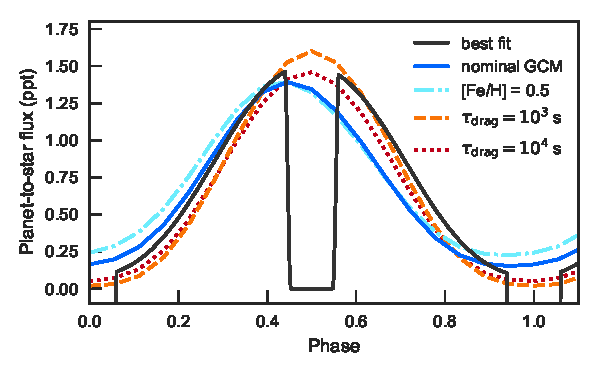
\includegraphics[width = 0.5\textwidth]{Figures/gcm_comparison.pdf}
\caption{GCM predictions (colored lines) compared to the best fit model for the WFC3 white light phase curve (black line). The nominal model is solar composition, cloud-free, with TiO/VO opacity and no drag. The models are multiplied by the predicted ellipsoidal variability of the planet.}
\label{fig:gcmcomparison}
\end{figure}

\begin{figure*}
	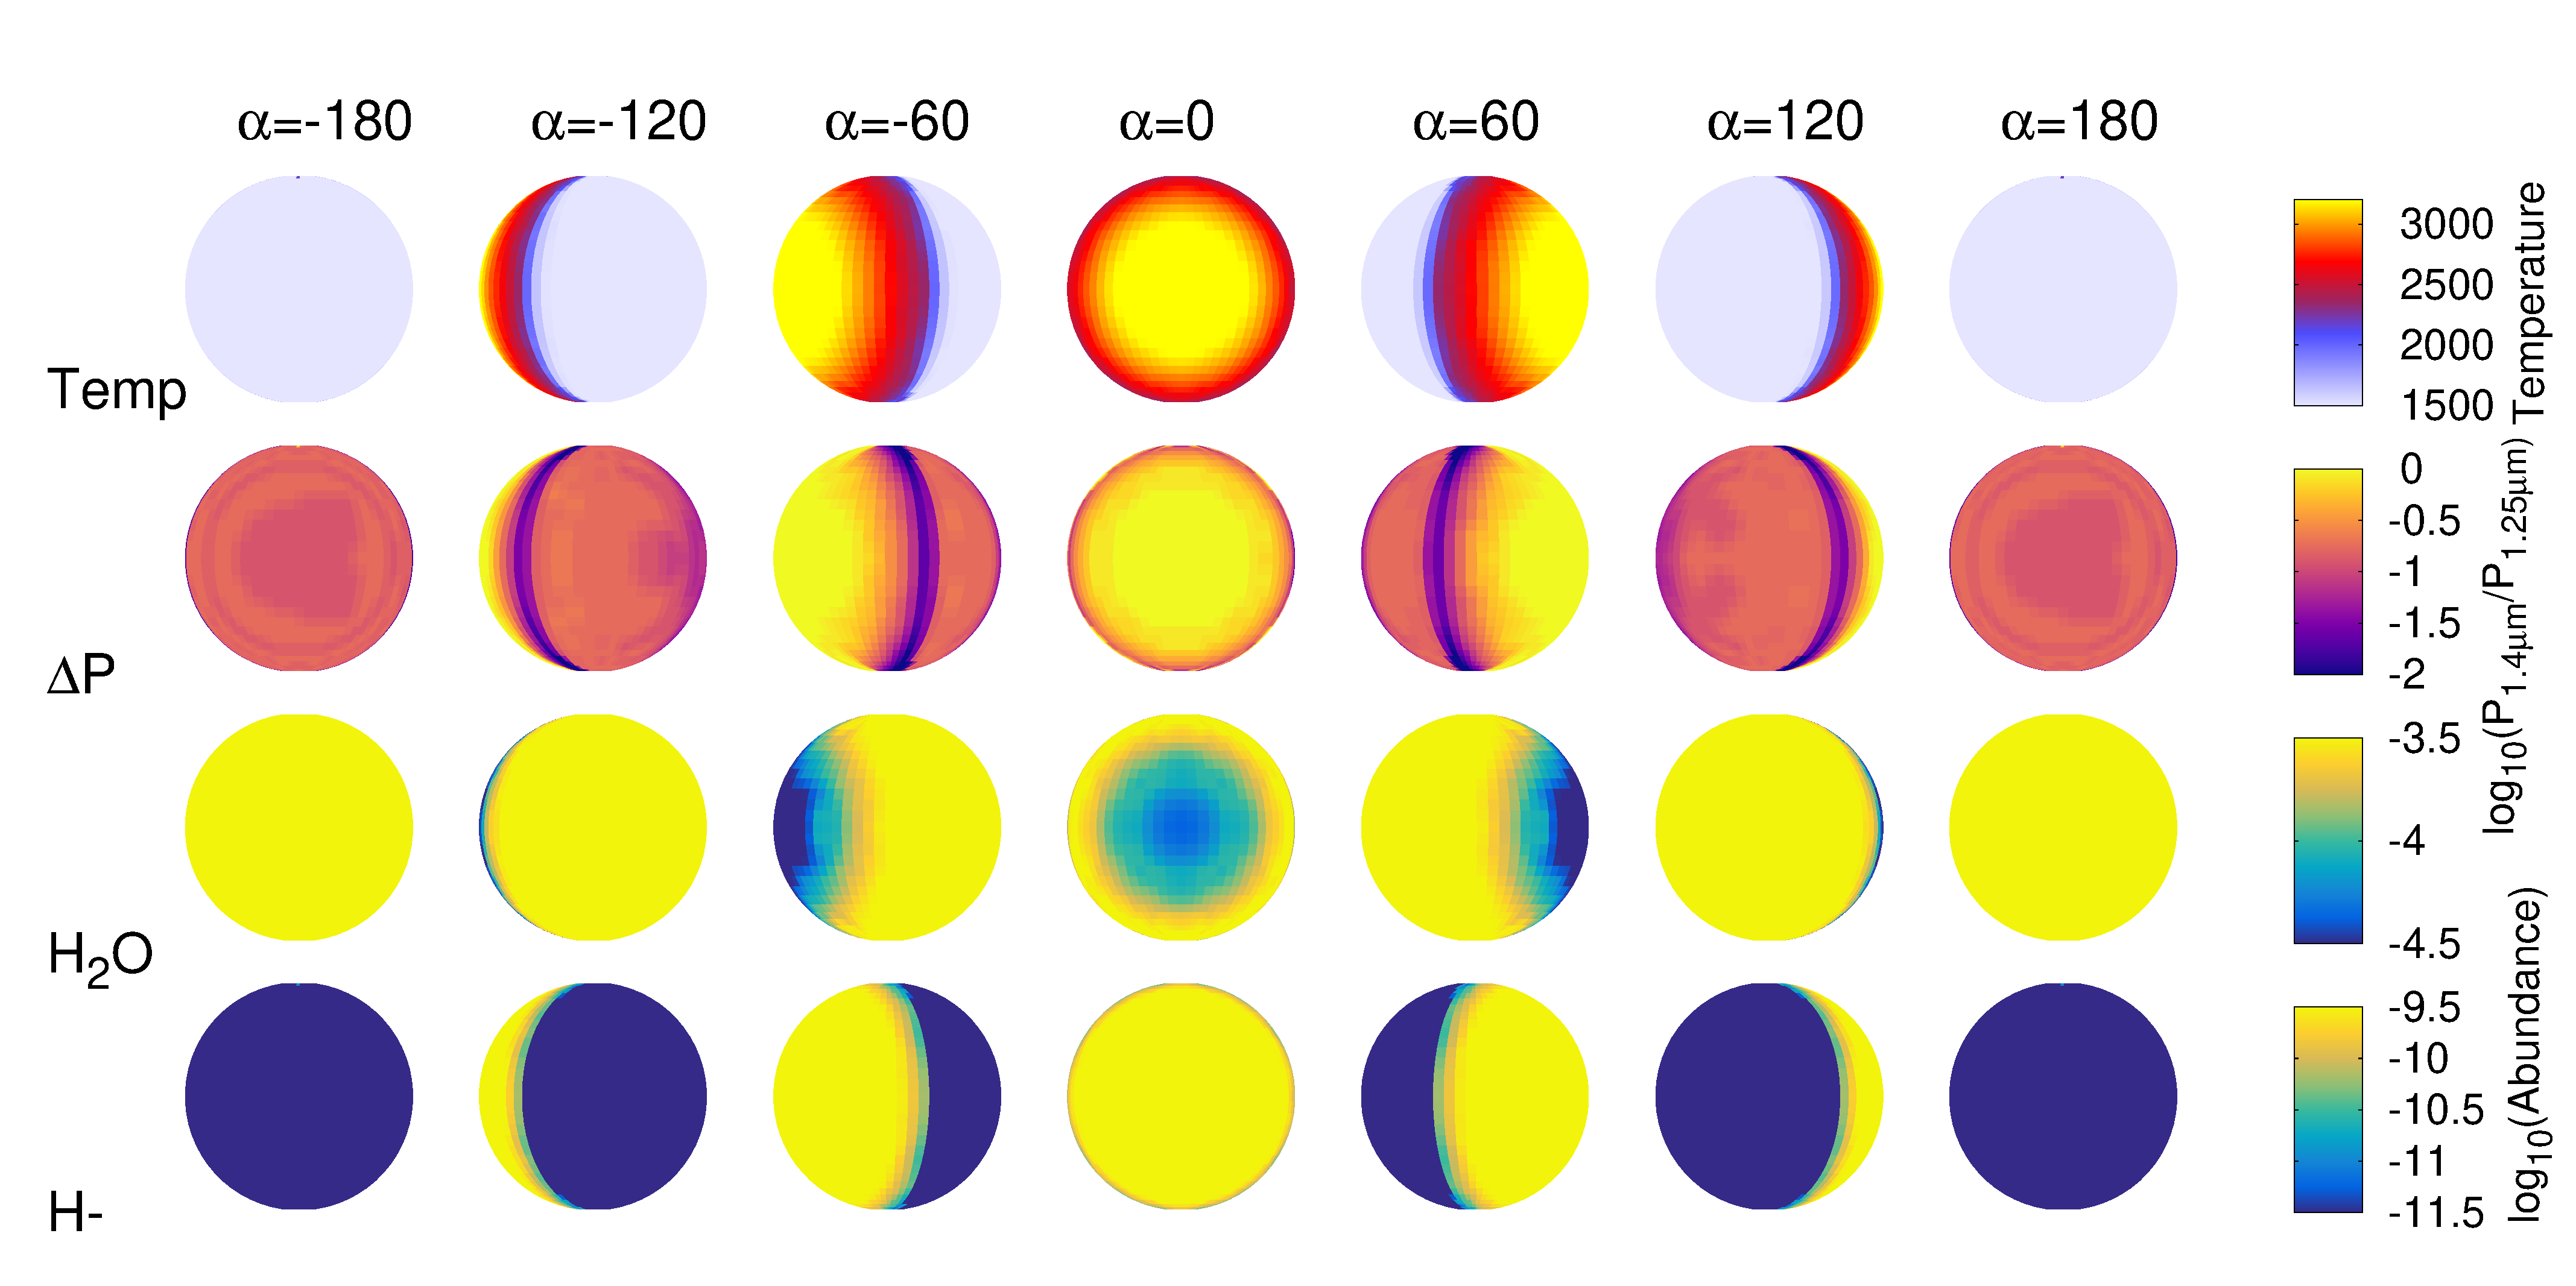
\includegraphics[width = 1.0\textwidth]{Figures/GCM_abundances.eps}
\caption{Abundances of key molecular species for different viewing geometries, from the $\tau_\mathrm{drag} = 10^3$ GCM.}
\label{fig:GCMabundance}
\end{figure*}


\section{Comparison with Brown Dwarfs and Directly Imaged Companions}
WASP-103b is so highly irradiated that its photospheric temperature ($2000 - 3000$ K) is comparable to that of low mass stars. However, the planet's other properties (surface gravity, rotation rate, irradiation) are different. To explore the effects of varying these parameters, we compared the spectra of WASP-103b to brown dwarfs and young directly imaged companions. 

We selected spectra from WASP-103b at three orbital phases: dayside ($\phi = 0.5$), quadrature ($\phi = 0.25$), and nightside ($\phi = 0.1$), and compared them to sources with comparable effective temperature. Figure\,\ref{fig:planetstarcomparison} shows the flux-calibrated spectra (assuming a distance of 10 pc).

The directly imaged spectra are taken from \cite{2008ApJ...689L.153L}, \cite{2010ApJ...719..497L}, \cite{2010A&A...512A..52B}, \cite{2011ApJ...729..139W} , \cite{2014A&A...562A.127B}, \cite{2011ApJ...730...42L}, \cite{2013ApJ...773...63A}, \cite{2016A&A...587A..56M}, \cite{2013ApJ...772...79A}, and \cite{2008ApJ...673L.185B}. They are calibrated\footnote{Apart for PZ Tel B whose flux calibration is detailed in \cite{2016A&A...587A..56M}.}in absolute flux using published H-band photometry \citep{2008ApJ...689L.153L, 2014A&A...562A.127B, 2011ApJ...729..139W, 2005A&A...430.1027C, 2011ApJ...730...42L, 2013ApJ...773...63A, 2003tmc..book.....C,2009A&A...506..799B} and distances \cite{2016A&A...595A...1G, 2007A&A...474..653V, 1999AJ....117..354D, 1999AJ....117.2381P}, a flux-calibrated spectrum of Vega \citep{1985A&A...151..399M, 1985IAUS..111..225H}, and the corresponding filter passbands.  The brown dwarf spectra \textbf{Jackie: describe catalog of brown dwarf spectra and flux calibration}.

The main spectral feature over the wavelength range we consider is water. To quantitatively compare the water feature amplitude for different objects, we define an amplitude $A = (R_\mathrm{1.3} - R_\mathrm{1.5})/F_\mathrm{1.3}$, where $F_\mathrm{X}$ is the average flux in a wavelength bin $0.1\,\mu$m wide centered on a wavelength $X$, and $R_\mathrm{X}$ is the bin-averaged residual from the best fit blackbody. These intervals were chosen such that all of the data have complete spectral coverage over the bin. 

%DI companions: 1RXSJ160929.1-210524b, J1610-1913B, TWA22A
%Age, logg, teff
%WASP-103b - logg = 3.2 



cite Tremblin et al. 2017 ? (https://arxiv.org/pdf/1710.02640.pdf)

\begin{figure*}
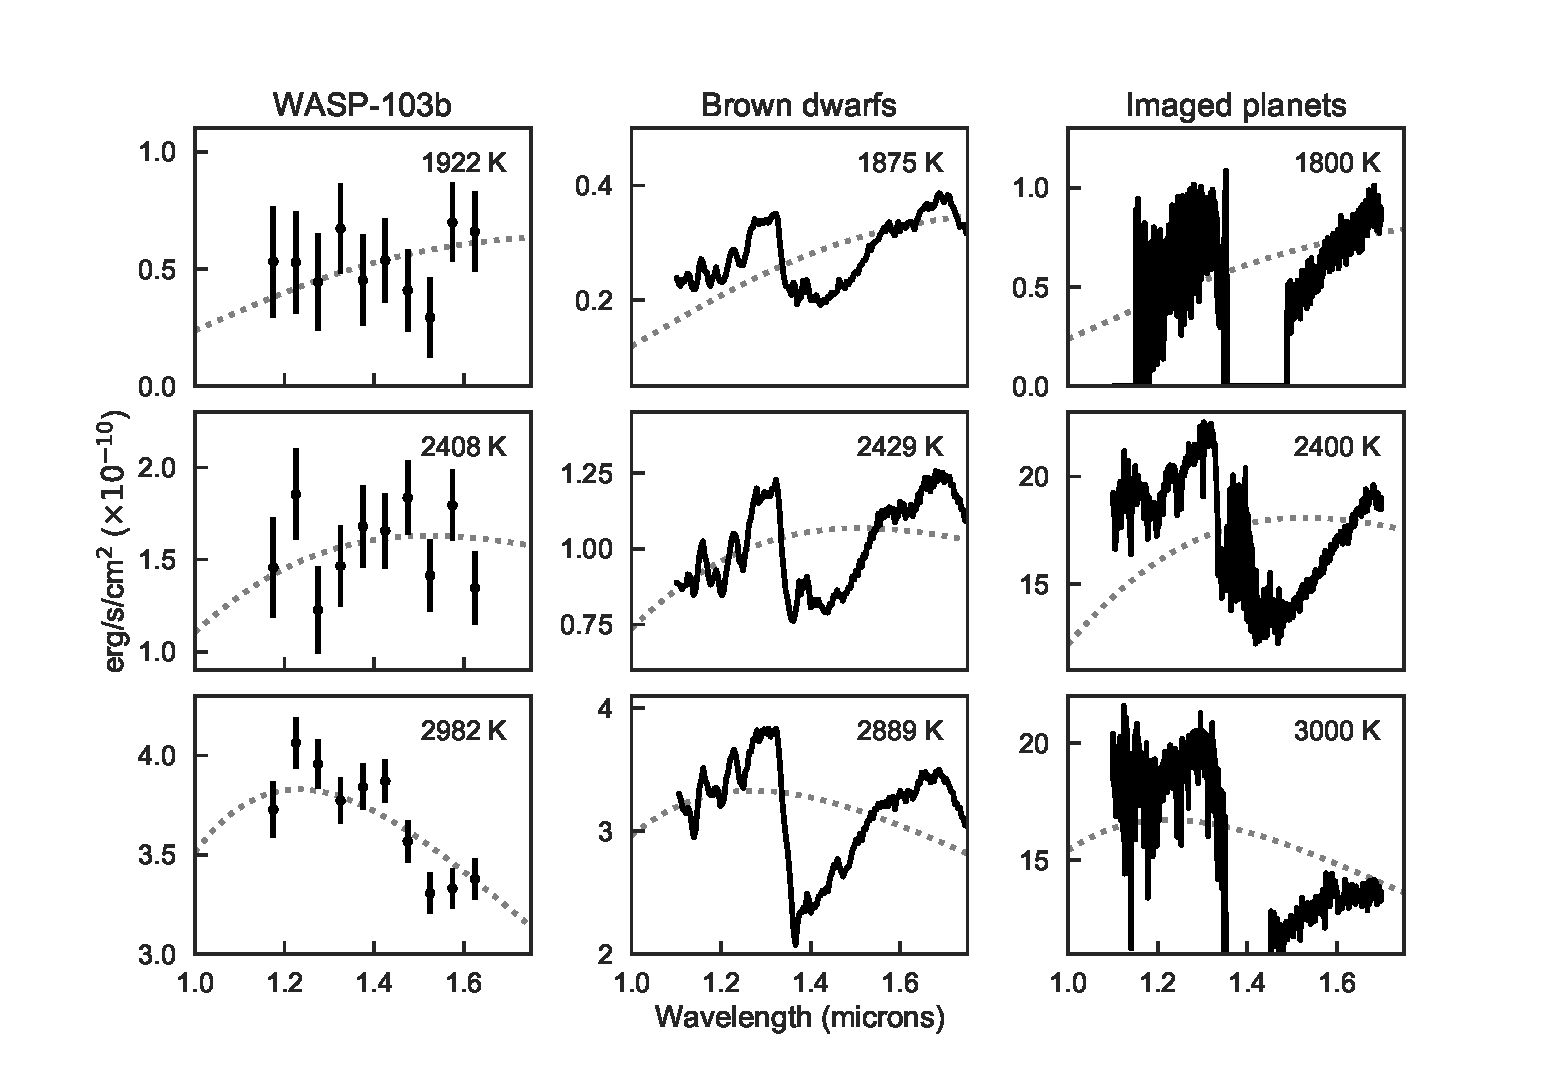
\includegraphics[width = 1.0\textwidth]{Figures/spectra_comparison.pdf}
\caption{Spectra for WASP-103b (left column) compared to brown dwarfs (middle) and directly imaged companions (right). The WASP-103b spectra are from the nightside (phase 0.1, top row), quadrature (phase 0.25, middle) and the dayside (phase 0.5, bottom). Each row shows spectra from objects of comparable temperature. The dotted gray line corresponds to the best fit blackbody. Effective temperatures are listed in the upper right corners.}
\label{fig:planetstarcomparison}
\end{figure*}

\section{Discussion and Conclusions}
One-dimensional retrieval is probably wrong, since we showed the dayside may have a large temperature gradient -> should work on this in the future.


There are many factors contributing to the blackbody spectra --
weak water xsec contrast, isothermal pt, H-, and dissociated water 


Cite Feng et al. 2016.

H- is important.

How does composition compare to other HJs.
The spectrum is similar to observations of several other ultra-hot Jupiters \citep[][]{arcangeli18, mansfield18}, but qualitatively different from slightly cooler planets, which show water absorption features in the near-infared \citep[e.g.][]{kreidberg14b, line16}.  

\acknowledgments
We thank a lot of people. Caroline Morley, Thomas Beatty, Ming Zhao, Kim Star Cartier, Hannah Diamond-Lowe, Nick Cowan (make him a coauthor?)

\bibliographystyle{aasjournal}
\bibliography{ms.bib}

\end{document}

